% TikZ 复刻。原图：assets/grating.png
% 回退：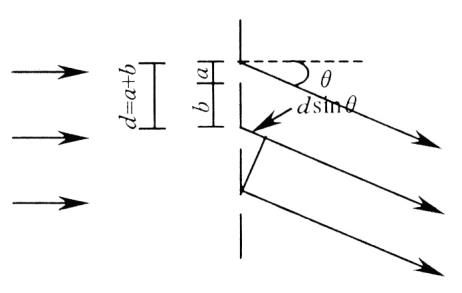
\includegraphics[width=0.62\linewidth]{assets/grating.png}
\begin{tikzpicture}[>=Stealth, font=\small]
  \def\W{5.4}
  \def\H{2.35}
  \def\slit{0.26}
  \def\barw{0.70}
  \fill[gray!65] (-\W/2,-\H/2) rectangle (\W/2,\H/2);
  \draw[thick] (-\W/2,-\H/2) rectangle (\W/2,\H/2);
  \foreach \k in {-2,-1,0,1,2} {
    \pgfmathsetmacro{\cx}{\k*(\slit+\barw)}
    \fill[white] (\cx-\slit/2,-\H/2+0.015) rectangle (\cx+\slit/2,\H/2-0.015);
  }
  \draw[<->] (-\slit/2,\H/2+0.32) -- (\slit/2,\H/2+0.32);
  \node[above=-1pt] at (0,\H/2+0.32) {$a$};
  \draw[<->] (\slit/2,\H/2+0.32) -- (\slit/2+\barw,\H/2+0.32);
  \node[above=-1pt] at ({\slit/2+\barw/2},\H/2+0.32) {$b$};
  \draw[dashed] (-\slit/2,-\H/2) -- (-\slit/2,-\H/2-0.58);
  \draw[dashed] (\slit/2+\barw,-\H/2) -- (\slit/2+\barw,-\H/2-0.58);
  \draw[<->] (-\slit/2,-\H/2-0.48) -- (\slit/2+\barw,-\H/2-0.48);
  \node[below] at ({(\barw)/2},-\H/2-0.48) {$d=a+b$};
\end{tikzpicture}
